\documentclass[12pt]{article}
\usepackage[utf8]{inputenc}
\usepackage[T1]{fontenc}
\usepackage{graphicx}
\usepackage{xcolor}
\usepackage{biblatex}
\addbibresource{example.bib}
%%novalidate

\usepackage{tikz}
\usepackage{calc}
\usepackage{booktabs}


% colors
\definecolor{color1}{HTML}{000060}
%\definecolor{color1}{HTML}{8C260F}
\definecolor{color2}{HTML}{333333}


% fonts
\usepackage{fontspec}
\defaultfontfeatures{Mapping=tex-text}
\setmainfont
[BoldFont=Lato-Bold.ttf,
ItalicFont=Lato-Italic.ttf,
BoldItalicFont=Lato-BoldItalic.ttf]
{Lato-Regular.ttf}
\newfontfamily\headingfont[ItalicFont=Lato-BlackItalic.ttf]{Lato-Black.ttf}
%%%

\usepackage{geometry}
\geometry{a4paper,
hmargin=20mm,vmargin=20mm,
head=0ex,foot=3ex}

\linespread{1.3}

\usepackage[hang]{caption}
\DeclareCaptionFormat{upper}{#1#2\uppercase{#3}\par}
\captionsetup{labelfont={bf,color=color2},textfont={normalsize,color=color2},format = upper,figurename=FIGURE,tablename=TABLE}

%%% fancy sections
\usepackage{titlesec}
%\titleformat{\chapter}{\headingfont\LARGE\bfseries\scshape\color{color1}}{\thechapter}{1em}{}[\titlerule]
\titleformat{\section}{\color{color1}\headingfont\Large\bfseries\uppercase}{\thesection}{1em}{}[\titlerule]
\titleformat{\subsection}{\color{color1}\headingfont\large\bfseries\uppercase}{\thesubsection}{1em}{}
\titleformat{\subsubsection}{\color{color1}\headingfont\bfseries\uppercase}{\thesubsubsection}{1em}{}
%%%

% head and foot
\usepackage{fancyhdr}
\pagestyle{fancy}
\lhead{}
\chead{}
\makeatletter
\rhead{\color{color2}\@date}
\makeatother
\newlength{\myheight}
\lfoot{
\settoheight{\myheight}{\thepage}
\raisebox{-2ex-0.5\myheight}{
\includegraphics[height=4ex]{logo}}
}
\cfoot{\color{color2}\ APC3}
\rfoot{\color{color2}\thepage}
\renewcommand\headrulewidth{0pt}
\renewcommand\footrulewidth{0pt}

% custom titlepage
\makeatletter
\newcommand*\DefVar[1]{\@namedef{#1}##1{\global\@namedef{get#1}{##1}}}
\DefVar{summary}
\renewcommand{\maketitle}{
\begin{center}

\begin{tikzpicture}
    \node[draw=none,%color1,line width=0.4pt,
      fill=color1,
      inner sep = 10pt,
      text width=\textwidth-20pt,
      text centered
    ] {\color{white}\headingfont\bfseries\huge\@title};
\end{tikzpicture}
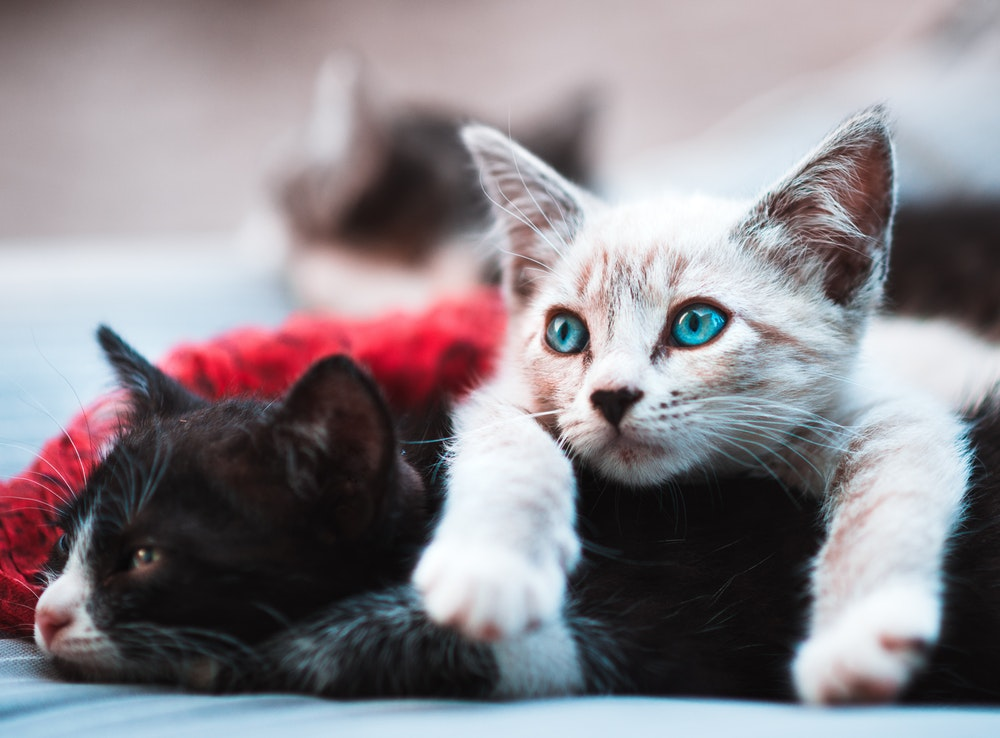
\includegraphics[width=\textwidth]{opening}\par
\headingfont\bfseries\Large\@author\par
\bigskip\medskip
{\color{color2}\normalfont\normalsize\textbf{Summary:}\\
\getsummary}
\end{center}
\clearpage
}
\makeatother
%%%

%%% fancy boxes
\usepackage{tcolorbox}
\usepackage{wrapfig}
\def\fullboxbegin{
\bigskip
\begin{tcolorbox}[colback=color1,colframe=color1,coltext=white,arc=0mm,boxrule=0pt]
}
\def\fullboxend{\end{tcolorbox}\medskip}
%
\def\leftboxbegin{
\begin{wrapfigure}{l}{0.5\textwidth}
\begin{tcolorbox}[colback=color1,colframe=color1,coltext=white,arc=0mm,boxrule=0pt]
}
\def\leftboxend{
\end{tcolorbox}
\end{wrapfigure}
}
%
\def\rightboxbegin{
\begin{wrapfigure}{r}{0.5\textwidth}
\begin{tcolorbox}[colback=color1,colframe=color1,coltext=white,arc=0mm,boxrule=0pt]
}
\def\rightboxend{
\end{tcolorbox}
\end{wrapfigure}
}
%
\newcounter{frames}
\def\frameboxbegin#1{
\bigskip
\refstepcounter{frames}
\begin{tcolorbox}[colback=white,colframe=color1,arc=0mm,title={\MakeUppercase{\textbf{Frame \arabic{frames}}: #1}}]
}
\def\frameboxend{
\end{tcolorbox}
}
%%%

\usepackage{lipsum}

%%%%%%%%%%%%%%%
% Title Page
\title{APC3 Assignment}
\author{Phoebe Liang}
\date{\today}
\summary{
Actuarial consultant providing advice to a general insurance company XYZ, which writes motor vehicle, home and contents, and building insurance policies. XYZ is expanding its policy offerings with a new product, electricity blackout insurance (EBI), to be made available to retail and commercial customers in Victoria. The committee is seeking advise on how this product would be structured and how it would be received by the customers. Furthermore, as part of its risk management strategy, the risk committee of XYZ is seeking advice in the use of electricity derivatives, so that they can report to the board on the feasibility of offering an electricity blackout insurance product.
}
%%%%%%%%%%%%%%%

\begin{document}
\maketitle

\tableofcontents
\clearpage

%%%%%%%%%%%%%%%
\section{Background}
\subsection{Electricity market in Australia}
\begin{flushleft}
The electricity system in Australia begins with acquisition of these primary energy sources: sunlight, wind, water, coal and gas.\parencite{aemc1} Historically, coal-fired power stations have played a dominating role in the electricity generation in Australia, but renewables such as sunlight, wind, water are growing rapidly to form a larger fraction of supply.\parencite{aer1} \par
\begin{figure}[!h]
  \centering
  \begin{minipage}[b]{0.45\textwidth}
    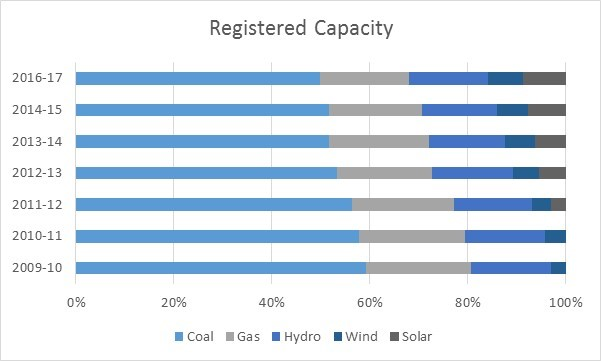
\includegraphics[width=\textwidth]{Registered_capacity.jpg}
    \caption{Registered Capacity}
  \end{minipage}
  \hfill
  \begin{minipage}[b]{0.45\textwidth}
    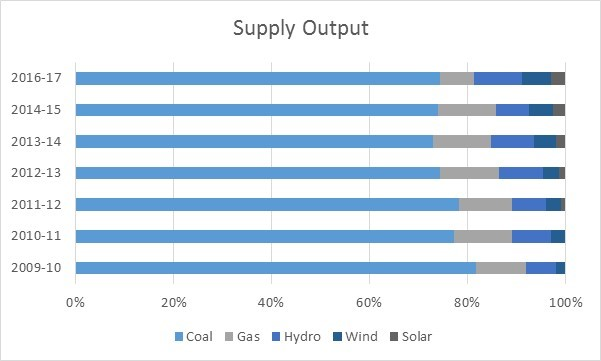
\includegraphics[width=\textwidth]{supply_output.jpg}
    \caption{Supply Output}
  \end{minipage}
\end{figure}
Then the generators make electricity from these sources and flows into the transmission network, which later transports electricity to the distribution network. The distribution network then transports electricity to residential and commercial buildings for end users.\parencite{aemc1} This is shown in the following figure. 
\begin{figure}[!h]
  \centering
  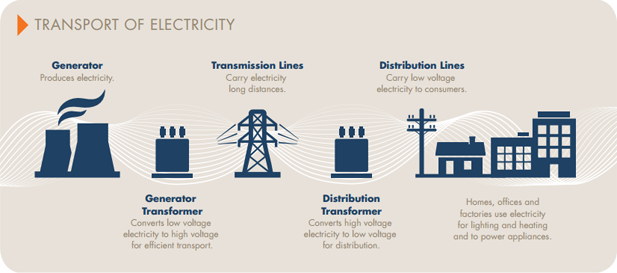
\includegraphics[width=\textwidth]{transport.png}
    \caption{Electricity Transport}
    \parencite{aemo1pic}
\end{figure}
\end{flushleft}
\newpage

\begin{flushleft}
The electricity market in Australia is made up of the:
\begin{itemize}
 \item competitive wholesale generation sector
 \item monopoly network business
 \item competitive retail sector\parencite{aemc2}
\end{itemize}
{\textbf{\large Competitive Wholesale Generation Sector:}}\par
The wholesale national electricity market (NEM) is where generators sell electricity to retailers so they can resell to businesses and households. There are 2 ways in trading electricity in NEM: through spot market or the contract market.\parencite{aemc2} The Australian Energy Market Commission (AEMC) overlooks the states and territories participating in NEM by developing and maintaining the Australian National Electricity Rules (NER). The rules are enforced by the Australian Energy Regulator (AER) and the day-to-day management of NEM is performed by the Australian Energy Market Operator (AEMO).\parencite{aemo1} \par
{\textbf{\large Monopoly Network Business:}}\par
The transmission and distribution networks are poles and wires, transformers, switches, monitoring equipment and everything that make up the electricity grid. Given the intensive investment to construct and manage the network, it is cost effective to have a monopoly network service.\parencite{aemc2}\par
{\textbf{\large Competitive Retail Sector:}}\par
In the retail sector, customers such as businesses and households buy electricity through retailers (e.g. Origin). Some large consumers such as manufactures may purchase electricity straight from wholesale market, i.e. through a generator rather than through a retailer.\parencite{aemc2} In this sector, electricity consumption by end users is distributed as the following:
\begin{figure}[!h]
  \centering
  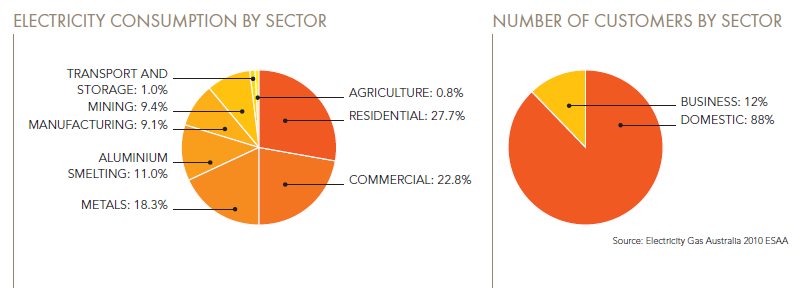
\includegraphics[width=\textwidth]{electricity_consumption.PNG}
    \caption{Electricity Transport}
    \parencite{aemo2}
\end{figure}
\end{flushleft}
\newpage

\subsection{Electricity blackout Compensation}
\begin{flushleft}
https://www.energy.vic.gov.au/safety-and-emergencies/power-outages/customer-compensation
start section here
\end{flushleft}

\subsection{Electricity Blackouts in Victoria}
\begin{flushleft}
start section here
\end{flushleft}
\newpage
%%%%%%%%%%%%%%%


%%%%%%%%%%%%%%%
\section{Product Structure}
\begin{flushleft}
Explain what EBI would seek to achieve for XYZ and its customers, describing a potential 
structure for the product and explaining the likelihood and severity of electricity blackouts in Victoria.
https://www.canstar.com.au/news-articles/power-outages-covered-home-insurance/ \par
Household: Food, AC, alarms? Can you make claims under the current policy? \par
Commercial: Loss of sales/efficiency, impact on bottom line? How to quantify these? Spike in electricity prices?\par
What are coverages? What can be claimed? How long?  
\end{flushleft}

\fullboxbegin
blor
\fullboxend
%%%%%%%%%%%%%%%


%%%%%%%%%%%%%%%
\section{Pricing and Risk}
Describe how the proposed product could be priced and the risks for the insurer XYZ. 

\leftboxbegin
formular in here?
\leftboxend

\lipsum[1]

\rightboxbegin
\begin{itemize}
 \item Lorem ipsum
 \item Lorem ipsum
\end{itemize}
\rightboxend

\lipsum[1]

\subsection{Pricing}
\lipsum[1]

\subsection{Risk}
\lipsum[1]
%%%%%%%%%%%%%%%


%%%%%%%%%%%%%%%
\section{Relevant Derivatives}
Outline the relevant derivative products offered on the Australian Stock Exchange, including how they are quoted and priced, paying particular attention to futures and options in respect of: 
\begin{itemize}
 \item Base - Quarterly
 \item Base - Monthly
 \item Base - Caps
 \item Base - Strip
 \item Peak - Quarterly
\end{itemize}
https://www.aemc.gov.au/energy-system/electricity/electricity-market/spot-and-contract-markets

\begin{table}[!h]
\centering
\caption{Sample table.}
\begin{tabular}{cccc}
\toprule
Value 1 & Value 2 & Value 3 & Value 4\\
\midrule
 odd     & odd   & odd & 1.00 \\
 even    & even  & even& 1.00 \\
 odd     & odd   & odd & 1.00 \\
 even    & even  & even& 1.00 \\
\bottomrule
\end{tabular}
\end{table}
%%%%%%%%%%%%%%%

%%%%%%%%%%%%%%%
\section{Liabilities Management}
Indicate how these could be used to manage XYZ’s EBI liabilities, giving a simple numerical example. \par

\frameboxbegin{Example: using derivatives to manage liabilities}
give a numerical example
\frameboxend
%%%%%%%%%%%%%%%

%%%%%%%%%%%%%%%
\section{Residual Risks Management}
Give some residual risks for XYZ and indicate how they could be managed. 
%%%%%%%%%%%%%%%

%%%%%%%%%%%%%%%
\section{Conclusion}
Give a conclusion on whether it is worthwhile XYZ pursuing an EBI offering, in whatever form. 
%%%%%%%%%%%%%%%

\printbibliography[heading=bibintoc]
\end{document}          
